\documentclass[KomodoMain.tex]{subfiles}
 
\begin{document}




\subsection{Demo Analysis}



\begin{table}[h]
\caption{Parameter settings}
\label{table:X}
\begin{tabular}{ p{1.75cm} p{1.4cm} p{1.4cm} p{1.75cm} p{1.5cm} p{2cm} p{2cm} }
 \hline
 Parameter   & $\omega_{min}$  & $\omega_{max}$ & $c_{1} = c_{2}$ & steps & \texttt{clamp\_pos} & \texttt{nhood\_size} \\
 \hline
 Value   & 0.7  & 0.3 &  1.496 & 100,000 & periodic & 5 \\
 \hline
\end{tabular}
\end{table}

The present value for $\omega_{min}$ is set as \texttt{PSO\_INERTIA} or 0.7. The strategy implemented is \texttt{PSO\_W\_LIN\_DEC}, which decreases the inertia weight. The settings control the degree of descent. \texttt{nhood\_size} denotes the number of informers for each particle, which in this case is 5.
\par
The demo was primarily analysed to examine the degree of premature convergence present in the algorithm itself. The tests were informed by the work on previous examinations of these specific benchmark functions \cite{funcs}. The program was executed for the purpose of testing using the \texttt{test.sh} bash file. Ten runs of each algorithm were performed for data collection. The \texttt{output.dat} files obtained were converted to \texttt{*.csv} for analysis.

\subsubsection{Search ranges}

\begin{table}[h]
\centering
\caption{Search ranges for each function}
\label{table:X}
\begin{tabular}{ |c c| }
 \hline
 Function   & Range \\
 \hline
 Ackley   & $-32.8, 32.8$  \\
 \hline
 Sphere & $-100, 100$ \\
 \hline
 Rosenbrock & $-2.048, 2.048$ \\
 \hline
 Griewank & $-600, 600$ \\
 \hline
\end{tabular}
\end{table}

The Ackley function has a global minimum of $f = 0$ where $x = (0, 0,...,0)$ though it has many minor local minima. 

\subsubsection{Analysis}

The first element will be to check the error achieved against the number of iterations of the algorithm required to achieve the desired margin of error. The second element of this analysis is to check the desired fitness level against the different levels actually achieved across different dimensions, \texttt{dim}. The mean fitness is the figure to look for. Note, mean time is quoted out of 25 runs. The standard deviation is the standard deviation between the mean values for each run, as explained below.

\begin{itemize}
\item \textbf{Best fitness:} This is the best fitness solution achieved by each benchmark function as represented by the minimum error level across all runs.
\item \textbf{Mean fitness:} This is the average figure for the fitness achieved over all runs by each benchmark function.
\item \textbf{Poorest fitness:} The least best fitness level achieved across all runs by each benchmark function.
\item \textbf{Standard deviation:} As mentioned, this is the standard deviation between the mean levels of fitness achieved in each individual run, aggregated for all runs.
\item \textbf{Mean time:} The average time taken for each run by each benchmark function.
\end{itemize}

\newpage
\begin{table}[!htbp]
\small
\caption{ \small Results for benchmark functions with dimensions $N = 20$, size = 18.}
\label{table:X}
\begin{tabular}{ p{3cm} p{2.4cm} p{2.4cm} p{2.4cm} p{2.4cm}}
 \hline
 Function   & Ackley  & Sphere & Rosenbrock & Griewank \\
 \hline
 Best fitness   & \textbf{2.6375E+00}  & \textbf{1.2000E+01} &  \textbf{0.0000E+00} & \textbf{4.1120E-01} \\
 
 Mean fitness & \textbf{5.3458E+00} & 1.2620E+03 & \textbf{7.0764E+02} & \textbf{1.0834E+01} \\
 
 Poorest fitness & \textbf{1.9595E+01} &  4.4634E+04 & \textbf{5.3914E+03} & \textbf{4.3180E+02} \\
 
 Standard deviation & \textbf{1.1635E-01} & \textbf{4.0254E+01} & 1.5574E+02 & \textbf{1.022E+00} \\
 
 Mean time (ms) & 120.40 & 71.20 & 108.40 & 130.80 \\
 \hline
\end{tabular}
\end{table}


\begin{table}[!htbp]
\small
\caption{\small Results for benchmark functions with dimensions $N = 30$, size = 20.}
\label{table:X}
\begin{tabular}{ p{3cm} p{2.4cm} p{2.4cm} p{2.4cm} p{2.4cm}}
 \hline
 Function   & Ackley  & Sphere & Rosenbrock & Griewank \\
 \hline
 Best fitness   & \textbf{3.276E+00} & 2.6000E+01 & \textbf{0.0000E+00} & \textbf{6.573E-01} \\
 
 Mean fitness & \textbf{5.8233E+00} & \textbf{1.6646E+03} & 3.1518E+03 & \textbf{1.4016E+01} \\
 
 Poorest fitness & \textbf{1.9640E+01} & 7.9735E+04 & \textbf{1.0195E+04} & \textbf{7.1847E+02} \\
 
 Standard deviation & \textbf{1.7158E-01} & \textbf{1.4613E+02} & 3.2299E+02 & \textbf{7.6188E-01} \\
 
 Mean time (ms) & 270.40 & 160.00 & 240.80 & 290.40 \\
 \hline
\end{tabular}
\end{table}


\begin{table}[!htbp]
\small
\caption{ \small Results for benchmark functions with dimensions $N = 50$, size = 24.}
\label{table:X}
\begin{tabular}{ p{3cm} p{2.4cm} p{2.4cm} p{2.4cm} p{2.4cm}}
 \hline
 Function   & Ackley  & Sphere & Rosenbrock & Griewank \\
 \hline
 Best fitness   & \textbf{4.0217E+00} & \textbf{7.8000E+01} &  3.8887E+03 & \textbf{8.9071E-01} \\
 
 Mean fitness & \textbf{6.931E+00} & \textbf{2.6504E+03} & 1.4254E+04 & \textbf{1.8769E+01} \\
 
 Poorest fitness & \textbf{1.9800E+01} & 1.4625E+05 & \textbf{1.8408E+04} & \textbf{1.245E+03} \\
 
 Standard deviation & \textbf{2.9957E-01} & \textbf{1.4614E+02} & 1.9429E+03 & \textbf{1.1489E+00} \\
 
 Mean time (ms) & 741.20 & 434.40 & 696.40 & 785.60 \\
 \hline
\end{tabular}
\end{table}


\begin{table}[!htbp]
\small
\caption{ \small Results for benchmark functions with dimensions $N = 70$, size = 26.}
\label{table:X}
\begin{tabular}{ p{3cm} p{2.4cm} p{2.4cm} p{2.4cm} p{2.4cm}}
 \hline
 Function   & Ackley  & Sphere & Rosenbrock & Griewank \\
 \hline
 Best fitness   & \textbf{4.9272E+00}  & \textbf{1.4500E+02} &  1.9924E+04 & \textbf{9.9511E-01} \\
 
 Mean fitness & \textbf{7.9936E+00} & \textbf{3.7159E+03} & 2.4221E+04 & \textbf{2.5144E+01} \\
 
 Poorest fitness & \textbf{1.9873E+01} & 2.0908E+05 & \textbf{2.7458E+04} & \textbf{1.8833E+03} \\
 
 Standard deviation & \textbf{2.8402E-01} & \textbf{2.4331E+02} & 1.9516E+03 & \textbf{1.2648E+00} \\
 
 Mean time (ms) & 1445.20 & 851.60 & 1394.80 & 1538.80 \\
 \hline
\end{tabular}
\end{table}


\begin{table}[!htbp]
\small
\caption{ \small Results for benchmark functions with dimensions $N = 100$, size = 30.}
\label{table:X}
\begin{tabular}{ p{3cm} p{2.4cm} p{2.4cm} p{2.4cm} p{2.4cm}}
 \hline
 Function   & Ackley  & Sphere & Rosenbrock & Griewank \\
 \hline
 Best fitness   & \textbf{6.0542E+00}  & \textbf{4.2000E+02} &  \textbf{2.9383E+04} & \textbf{1.1134E+00} \\
 
 Mean fitness & \textbf{9.4993E+00} & 6.0538E+03 & 3.5019E+04 & \textbf{3.2981E+01} \\
 
 Poorest fitness & \textbf{1.9894E+01} & \textbf{3.0353E+05} & \textbf{4.5821E+04} & \textbf{2.7054E+03} \\
 
 Standard deviation & \textbf{4.1190E-01} & 4.3564E+02 & 3.6994E+03 & \textbf{1.3156E+00} \\
 
 Mean time (ms) & 2908.00 & 1819.60 & 2831.20 & 3194.00 \\
 \hline
\end{tabular}
\end{table}

\begin{table}[!htbp]
\small
\caption{ \small Results for benchmark functions with dimensions $N = 500$, size = 54.}
\label{table:X}
\begin{tabular}{ p{3cm} p{2.4cm} p{2.4cm} p{2.4cm} p{2.4cm}}
 \hline
 Function   & Ackley  & Sphere & Rosenbrock & Griewank \\
 \hline
 Best fitness  & 1.4433E+01 & 5.7015E+04 & 1.9829E+05 & 4.8773E+01  \\
 
 Mean fitness & 1.6645E+01 & 1.3874E+05 & 2.1792E+05 & 3.0480E+02 \\
 
 Poorest fitness & 1.9972E+01 & 1.5935E+06 & 2.2998E+05 & 1.4501E+04\\
 
 Standard deviation & 6.1797E-01 & 2.7717E+04 & 6.9748E+03 & 7.1154E+01 \\
 
 Mean time (ms) & 147818.00 & 95558.40 & 74689.60 & 134804.80\\
 \hline
\end{tabular}
\end{table}

\begin{table}[!htbp]
\small
\caption{\small Results for benchmark functions with dimensions $N = 1000$, size = 73.}
\label{table:X}
\begin{tabular}{ p{3cm} p{2.4cm} p{2.4cm} p{2.4cm} p{2.4cm}}
 \hline
 Function   & Ackley  & Sphere & Rosenbrock & Griewank \\
 \hline
 Best fitness   & 1.7250E+01 & 3.2513E+05 & 4.3102E+05 &  7.3685E+02 \\
 
 Mean fitness & 1.8593E+01 & 5.7175E+05 & 4.5025E+05 & 1.6362E+03 \\
 
 Poorest fitness & 1.9993E+01 & 3.2470E+06 & 4.6860E+05 & 2.9311E+04 \\
 
 Standard deviation & 3.2277E-01 & 1.1247E+05 & 1.0289E+04 & 3.2838E+02 \\
 
 Mean time (ms) & 560022.80 & 419196.80 & 299853.20 & 590098.00 \\
 \hline
\end{tabular}
\end{table}


\newpage

\begin{figure}[!htbp]
\caption{Standard deviations of the means illustrate the break in consistency with the Rosenbrock benchmark.}
\centering
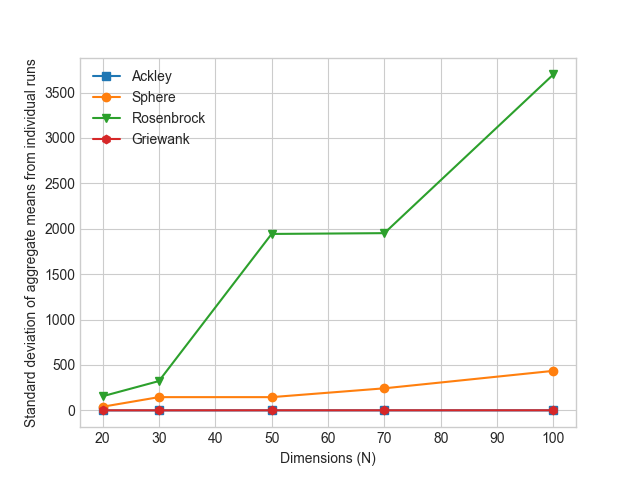
\includegraphics[width=0.9\textwidth]{stdev.png}
\end{figure}

\begin{figure}[!htbp]
\caption{Standard deviations of the means up to $N = 1000$.}
\centering
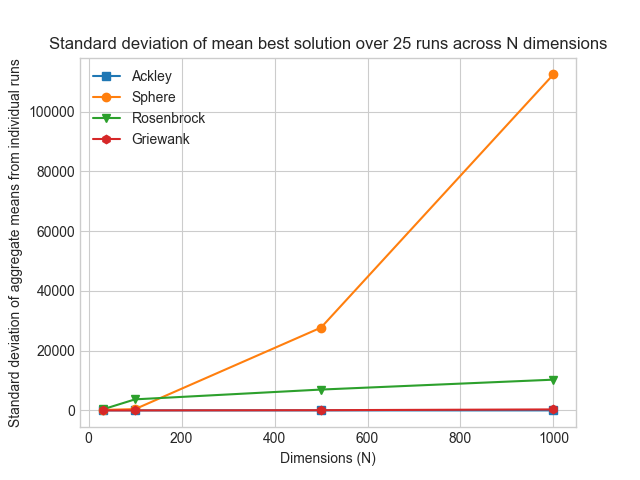
\includegraphics[width=0.9\textwidth]{Figure_n1000.png}
\end{figure}

\newpage

\subsubsection{Timing Graphs}

\begin{figure}[!htbp]
\caption{Average time per run for each function.}
\centering
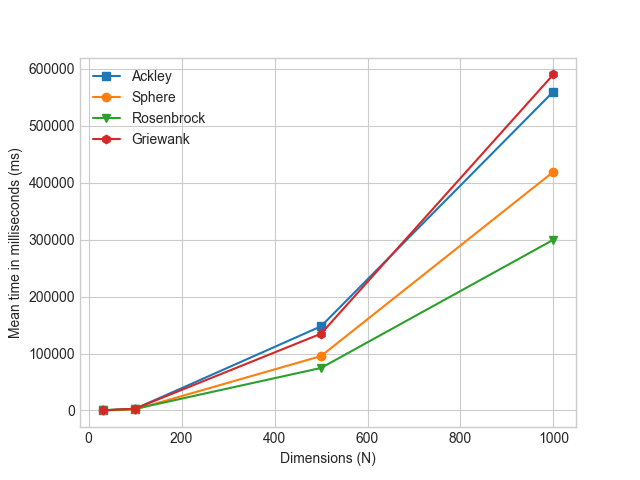
\includegraphics[width=0.9\textwidth]{demo_timings.png}
\end{figure}

\newpage
\subsubsection{Convergence Graphs}

\begin{figure}[!htbp]
     \centering
     \begin{subfigure}[b]{0.4\textwidth}
         \centering
         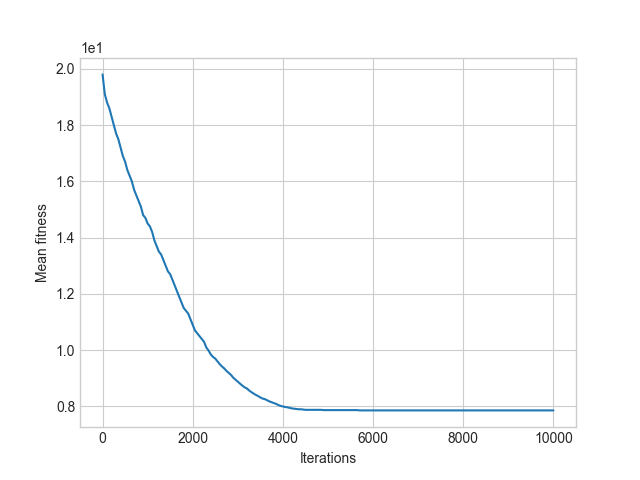
\includegraphics[width=\textwidth]{ackley100.png}
         \caption{Ackley}
         \label{fig:ackley}
     \end{subfigure}
     \hfill
     \begin{subfigure}[b]{0.4\textwidth}
         \centering
         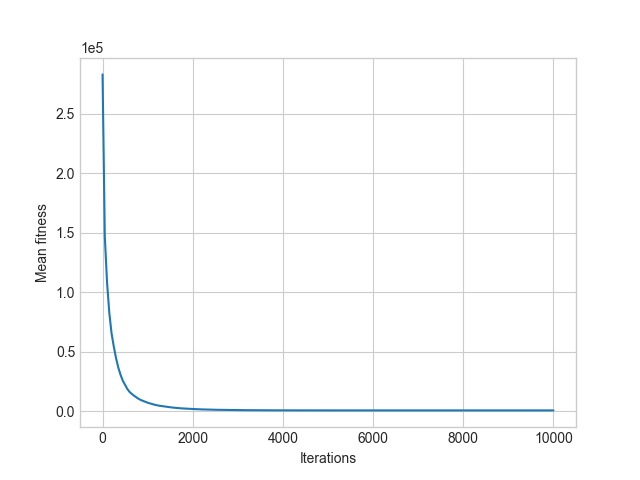
\includegraphics[width=\textwidth]{sphere100.png}
         \caption{Sphere}
         \label{fig:sphere}
     \end{subfigure}
     \hfill
     \begin{subfigure}[b]{0.4\textwidth}
         \centering
         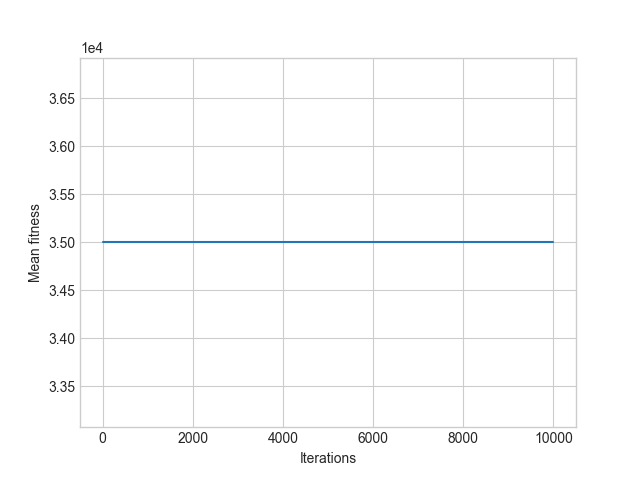
\includegraphics[width=\textwidth]{rosenbrock100.png}
         \caption{Rosenbrock}
         \label{fig:rosenbrock}
     \end{subfigure}
     \hfill
     \begin{subfigure}[b]{0.4\textwidth}
         \centering
         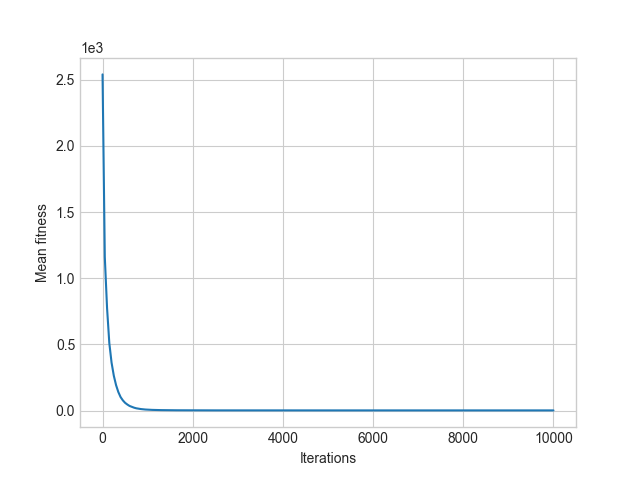
\includegraphics[width=\textwidth]{griewank100.png}
         \caption{Griewank}
         \label{fig:griewank}
     \end{subfigure}
        \caption{Convergence graphs for each function at $N = 100$ dimensions.}
        \label{fig:four graphs}
\end{figure}


\newpage
\subsection{Discussion of observations}  

\subsubsection{Ackley}

In terms of timing, Ackley is fine with 20 and 30 dimensions, but then begins to decay, coming second only to Griewank. That being said, the mean fitness levels achieved are consistently the best out of the benchmark set and even the poorer fitness levels cannot compare with even the better Rosenbrock or Sphere ones in the higher dimensions. The standard deviation between the mean best fitness levels achieved per run (see Figure 1) are also comparatively the lowest.

\subsubsection{Sphere}

The Sphere function is dependable in lower dimensions and doesn't decay too much in terms of time. This function does however achieve the poorest fitness levels once $N$ is greater than $30$. Whilst the means achieved do not deviate as much as those achieved by the Rosenbrock function, it is nonetheless prone to break in terms of deviations earlier.

\subsubsection{Rosenbrock}

Rosenbrock is not well behaved in the higher dimensions in spite of its better performance measures at the lower dimensions. A quick median fitness analysis for Rosenbrock at $N=30$ is 0.77712, so it converges very quickly in lower dimensions. Time decay takes hold when $N=70$, and so it does not achieve the correct fitness levels afterwards.

\subsubsection{Griewank}

Griewank decayed the most in terms of timing. Less deviation between the average time of each run for each function due to higher computational load and the sort mechanism in memory is the case here, since the function, whilst able to achieve a consistent fitness level, can also encounter much poorer fitness levels when in the process of evaluating.

\newpage

\subsection{Next steps}

The next step will be to run these same tests in parallel to see what the performance improvement is by adjusting the number of processors. With the path planning problem, the serial evaluation will look at how increasing the number of particles affects performance, and thus with the parallel evaluation of that application, the same assessment will take place, but with the spread of N particles across multiple processors. The appendix will be further developed to accommodate more graphical analysis that cannot be included in the main body of the report.

\subsection{Increment and Problem Dimensionality}

\lstinputlisting[language=C, caption=Function for calculating appropriate swarm size]{pso_calc_swarm_size.c}

All of the demo runs were performed with swarm sizes that were less than 100, with the highest, $N = 1000$ containing a swarm size of 73. An automatic calculation of the swarm size was performed by the function shown above, which was used in each case. The classical thinking on the population size is that the best performance typically occurs in populations with smaller sizes, hence the restricted allowance for incrementation with the problem dimensions. However, it has been argued recently that the smaller sizes selected to evaluated different optimisation problems may indeed be too small \cite{ssize}. 
\par
The authors of this paper have argued that the best results are typically obtained in the 70-500 size range. This is not a problem for the results obtained above as the range of sizes is incremented sufficiently, and evaluation of the impact of higher dimensions versus the increased population size is beyond the scope of this analysis. Nonetheless, it is evident that the impact of higher dimensions likely outweighs any influence a population size beyond 100 would have, as can be seen by the breakdown in performance of the Rosenbrock benchmark.


\subsection{Profiling}

X

\subsection{PSO Topologies}

X

\end{document}